\chapter{Lecture 2}

%--- 信息 ----
\begin{center}
    讲师:王立威 \qquad
    课程时间:25.Feb.25th \qquad 
    笔记:25.June.7th
\end{center}

\bigskip

首先,我们不失一般性地考虑如下的通讯需求:
\begin{itemize}
    \item 无限次的通信(infinite communication)
    \item 信息服从某个固定分布(A prob. distribution over the messages)
\end{itemize}

在这样的背景下,我们力求最小化平均编码长度. 

注意到,我们为了接收方可以唯一解码,我们考虑一组无前缀码(Prefix-Free Codes). 值得注意,这只是一个充分条件,而并不是必要条件.  (下面的例子中就可以看出)
\begin{example}
    考虑码字为$\{0, 01\}$,这并不是无前缀的,但可以唯一解码. 
\end{example}

但事实上,考虑可唯一译码,可以归约到考虑无前缀码,这是由如下的定理保证的:
\begin{theorem}
    记$A$表示所有无前缀码,$B$表示所有可唯一译码,显然有$A\sbne B$.  用$l(C,m)$表示使用码$C$编译信息$m$时的码长,那么可以证明 
    \[
    \min_{C\in B} \E_{m \sim P}\Big[l(C,m)\Big] = \min_{C\in A} \E_{m \sim P}\Big[l(C,m)\Big]
    \]
\end{theorem}
\begin{proof}
    此略去. 主要思想是证明对于任意$C^* \in B$使得$\E l(C^*)$达到最小值,都存在一个对应的$\tilde{C}^* \in A$使得$\E l(\tilde{C}^*) = \E l(C^*)$.  
\end{proof} 

有了上面的基础理论,我们来尝试求无前缀码的最短平均码长。 首先,Kraft不等式为我们估计了一个下界.
\begin{theorem}[无前缀码的Kraft不等式]
    假设码$C=(c_1,\dots,c_n)$是无前缀的,记$l_1,\dots, l_n$分别是$c_1,\dots, c_n$的长度(此指比特数),则 
    \[
    \sum_{i=1}^n 2^{-l_i} \le 1
    \]
\end{theorem} 
\begin{proof}
    这个定理的证明是简单的,构造一棵二叉树,根据码的内容嵌入该二叉树。由于$C$是无前缀码,所以不存在一个码对应的结点是另一个码对应的节点的祖先。故所有码$c_i$都在叶结点上,再归纳地证明满二叉树叶节点的$\sum 2^{-d_i} = 1$即可.
\end{proof}

接下来,我们给定信息为$M = \{m_1, \dots, m_n\}$,对应的分布列为$P = (p_1, \dots, p_n)$,其中$p_i = \Pr[m_i]$。 我们的目标是找到一个无前缀码$C = (c_1,\dots, c_n)$,其长度为$l_1,\dots,l_n$。使得平均码长最短,可见这事实上是一个优化问题:
\begin{align*}
    \minimize_l \ & \sum_{i=1}^n p_i l_i  \\
    \text{s.t.} \ & \sum_{i=1}^n 2^{-l_i} \le 1\\
    & l_i \in \N , i=1,2,\dots,n
\end{align*}

但这样的问题还是有些复杂,我们不妨去掉整数的约束,并且直接限定Kraft不等式中等号成立:
\begin{align*}
    \minimize_l \ & \sum_{i=1}^n p_i l_i  \\
    \text{s.t.} \ & \sum_{i=1}^n 2^{-l_i} = 1\\
    & l_i \ge 0 , i=1,2,\dots,n
\end{align*}

使用Jensen不等式或Lagrange乘子法(此略去)易得 
\[
\min_l \sum_{i=1}^n p_i l_i = \sum_{i=1}^n p_i \log_2 1/p_i
\]

由此延伸出\textbf{熵}的定义:
\begin{definition}[熵]
    给定随机元$X$,及其分布列$(p_1, \dots, p_n)$,定义$X$的\textbf{信息熵}(entropy)为 
    \[
    H(X) := \sum_{i=1}^n p_i \log_2 1/p_i = - \sum_{i=1}^n p_i \log_2 p_i
    \]
\end{definition}

在不导致歧义的情况下,可以简称信息熵为熵。这个量有如下意义和特性:
\begin{itemize}
    \item 最短编码长度,即描述该变量所需的长度下界
    \item 量化了“信息”这一概念
    \item 均匀分布时$H(X)$最大(最不确定,无先验),而退化分布时$H(X)=0$ 
    \item 度量了$X$的不确定性
\end{itemize}

$n=2$时:
\begin{figure}[H]
    \centering
    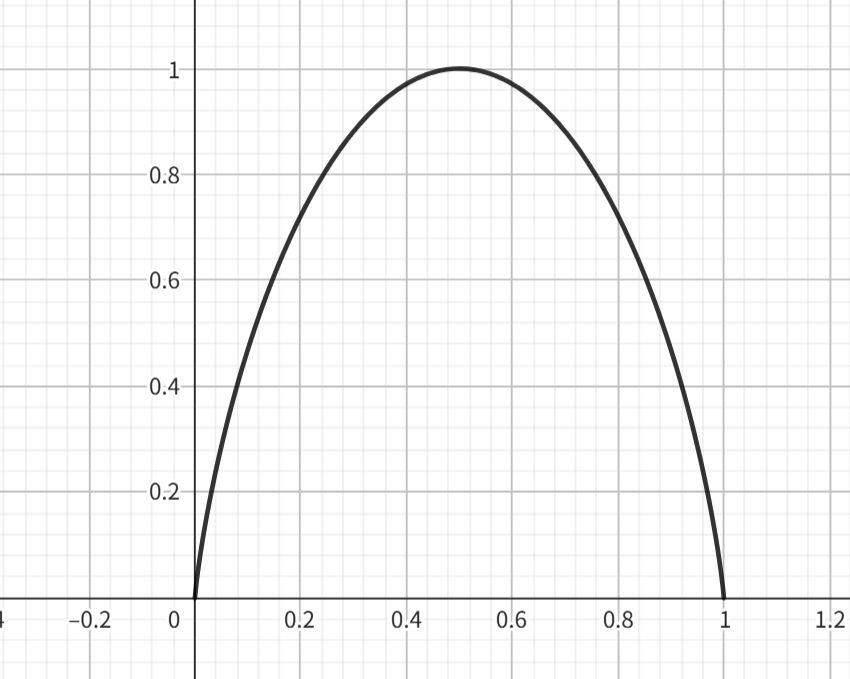
\includegraphics[width=.6\textwidth]{images/c2_1.png}
    \caption{$H=x\log 1/x + (1-x)\log 1/(1-x)$的图像}
\end{figure}